\documentclass[paper=letter,11pt]{scrartcl}

\KOMAoptions{headinclude=true, footinclude=false}
\KOMAoptions{DIV=14, BCOR=5mm}
\KOMAoptions{numbers=noendperiod}
\KOMAoptions{parskip=half}
\addtokomafont{disposition}{\rmfamily}
\addtokomafont{part}{\LARGE}
\addtokomafont{descriptionlabel}{\rmfamily}
%\setkomafont{pageheadfoot}{\normalsize\sffamily}
\setkomafont{pagehead}{\normalsize\rmfamily}
%\setkomafont{publishers}{\normalsize\rmfamily}
\setkomafont{caption}{\normalfont\small}
\setcapindent{0pt}
\deffootnote[1em]{1em}{1em}{\textsuperscript{\thefootnotemark}\ }


\usepackage{amsmath}
\usepackage[varg]{txfonts}
\usepackage[T1]{fontenc}
\usepackage{graphicx}
\usepackage{xcolor}
\usepackage[american]{babel}
% hyperref is needed in many places, so include it here
\usepackage{hyperref}

\usepackage{xspace}
\usepackage{multirow}
\usepackage{float}


\usepackage{braket}
\usepackage{bbm}
\usepackage{relsize}
\usepackage{tcolorbox}

\def\ketY{\ensuremath{\ket {\Psi}}}
\def\iGeV{\ensuremath{\textrm{GeV}^{-1}}}
%\def\mp{\ensuremath{m_{\textrm{proton}}}}
\def\rp{\ensuremath{r_{\textrm{proton}}}}
\def\me{\ensuremath{m_{\textrm{electron}}}}
\def\aG{\ensuremath{\alpha_G}}
\def\rAtom{\ensuremath{r_{\textrm{atom}}}}
\def\rNucl{\ensuremath{r_{\textrm{nucleus}}}}
\def\GN{\ensuremath{\textrm{G}_\textrm{N}}}
\def\ketX{\ensuremath{\ket{\vec{x}}}}
\def\ve{\ensuremath{\vec{\epsilon}}}


\def\ABCDMatrix{\ensuremath{\begin{pmatrix} A &  B  \\ C  & D \end{pmatrix}}}
\def\xyprime{\ensuremath{\begin{pmatrix} x' \\ y' \end{pmatrix}}}
\def\xyprimeT{\ensuremath{\begin{pmatrix} x' &  y' \end{pmatrix}}}
\def\xy{\ensuremath{\begin{pmatrix} x \\ y \end{pmatrix}}}
\def\xyT{\ensuremath{\begin{pmatrix} x & y \end{pmatrix}}}

\def\IMatrix{\ensuremath{\begin{pmatrix} 0 &  1  \\ -1  & 0 \end{pmatrix}}}
\def\IBoostMatrix{\ensuremath{\begin{pmatrix} 0 &  1  \\ 1  & 0 \end{pmatrix}}}
\def\JThree{\ensuremath{\begin{pmatrix}    0 & -i & 0  \\ i & 0  & 0 \\ 0 & 0 & 0 \end{pmatrix}}} 
\def\JTwo{\ensuremath{\begin{bmatrix}    0 & 0 & -i  \\ 0 & 0  & 0 \\ i & 0 & 0 \end{bmatrix}}}
\def\JOne{\ensuremath{\begin{bmatrix}    0 & 0 & 0  \\ 0 & 0  & -i \\ 0 & i & 0 \end{bmatrix}}}
\def\etamn{\ensuremath{\eta_{\mu\nu}}}
\def\Lmn{\ensuremath{\Lambda^\mu_\nu}}
\def\dmn{\ensuremath{\delta^\mu_\nu}}
\def\wmn{\ensuremath{\omega^\mu_\nu}}
\def\be{\begin{equation*}}
\def\ee{\end{equation*}}
\def\bea{\begin{eqnarray*}}
\def\eea{\end{eqnarray*}}
\def\bi{\begin{itemize}}
\def\ei{\end{itemize}}
\def\fmn{\ensuremath{F_{\mu\nu}}}
\def\fMN{\ensuremath{F^{\mu\nu}}}
\def\bc{\begin{center}}
\def\ec{\end{center}}
\def\nus{$\nu$s}

\def\adagger{\ensuremath{a_{p\sigma}^\dagger}}
\def\lineacross{\noindent\rule{\textwidth}{1pt}}

\newcommand{\multiline}[1] {
\begin{tabular} {|l}
#1
\end{tabular}
}

\newcommand{\multilineNoLine}[1] {
\begin{tabular} {l}
#1
\end{tabular}
}



\newcommand{\lineTwo}[2] {
\begin{tabular} {|l}
#1 \\
#2
\end{tabular}
}

\newcommand{\rmt}[1] {
\textrm{#1}
}


%
% Units
%
\def\m{\ensuremath{\rmt{m}}}
\def\GeV{\ensuremath{\rmt{GeV}}}
\def\pt{\ensuremath{p_\rmt{T}}}


\def\parity{\ensuremath{\mathcal{P}}}

\usepackage{cancel}
\usepackage{ mathrsfs }
\def\bigL{\ensuremath{\mathscr{L}}}

\usepackage{ dsfont }



\usepackage{fancyhdr}
\fancyhf{}

%\documentclass[margin,line]{res}
\usepackage{braket}
\usepackage{bbm}
\usepackage{relsize}
\usepackage{tcolorbox}


\def\ketY{\ensuremath{\ket {\Psi}}}
\def\iGeV{\ensuremath{\textrm{GeV}^{-1}}}
%\def\mp{\ensuremath{m_{\textrm{proton}}}}
\def\rp{\ensuremath{r_{\textrm{proton}}}}
\def\me{\ensuremath{m_{\textrm{electron}}}}
\def\aG{\ensuremath{\alpha_G}}
\def\rAtom{\ensuremath{r_{\textrm{atom}}}}
\def\rNucl{\ensuremath{r_{\textrm{nucleus}}}}
\def\GN{\ensuremath{\textrm{G}_\textrm{N}}}
\def\ketX{\ensuremath{\ket{\vec{x}}}}
\def\ve{\ensuremath{\vec{\epsilon}}}


\def\ABCDMatrix{\ensuremath{\begin{pmatrix} A &  B  \\ C  & D \end{pmatrix}}}
\def\xyprime{\ensuremath{\begin{pmatrix} x' \\ y' \end{pmatrix}}}
\def\xyprimeT{\ensuremath{\begin{pmatrix} x' &  y' \end{pmatrix}}}
\def\xy{\ensuremath{\begin{pmatrix} x \\ y \end{pmatrix}}}
\def\xyT{\ensuremath{\begin{pmatrix} x & y \end{pmatrix}}}

\def\IMatrix{\ensuremath{\begin{pmatrix} 0 &  1  \\ -1  & 0 \end{pmatrix}}}
\def\IBoostMatrix{\ensuremath{\begin{pmatrix} 0 &  1  \\ 1  & 0 \end{pmatrix}}}
\def\JThree{\ensuremath{\begin{pmatrix}    0 & -i & 0  \\ i & 0  & 0 \\ 0 & 0 & 0 \end{pmatrix}}} 
\def\JTwo{\ensuremath{\begin{bmatrix}    0 & 0 & -i  \\ 0 & 0  & 0 \\ i & 0 & 0 \end{bmatrix}}}
\def\JOne{\ensuremath{\begin{bmatrix}    0 & 0 & 0  \\ 0 & 0  & -i \\ 0 & i & 0 \end{bmatrix}}}
\def\etamn{\ensuremath{\eta_{\mu\nu}}}
\def\Lmn{\ensuremath{\Lambda^\mu_\nu}}
\def\dmn{\ensuremath{\delta^\mu_\nu}}
\def\wmn{\ensuremath{\omega^\mu_\nu}}
\def\be{\begin{equation*}}
\def\ee{\end{equation*}}
\def\bea{\begin{eqnarray*}}
\def\eea{\end{eqnarray*}}
\def\bi{\begin{itemize}}
\def\ei{\end{itemize}}
\def\fmn{\ensuremath{F_{\mu\nu}}}
\def\fMN{\ensuremath{F^{\mu\nu}}}
\def\bc{\begin{center}}
\def\ec{\end{center}}
\def\nus{$\nu$s}

\def\adagger{\ensuremath{a_{p\sigma}^\dagger}}
\def\lineacross{\noindent\rule{\textwidth}{1pt}}

\newcommand{\multiline}[1] {
\begin{tabular} {|l}
#1
\end{tabular}
}

\newcommand{\multilineNoLine}[1] {
\begin{tabular} {l}
#1
\end{tabular}
}



\newcommand{\lineTwo}[2] {
\begin{tabular} {|l}
#1 \\
#2
\end{tabular}
}

\newcommand{\rmt}[1] {
\textrm{#1}
}


%
% Units
%
\def\m{\ensuremath{\rmt{m}}}
\def\GeV{\ensuremath{\rmt{GeV}}}
\def\pt{\ensuremath{p_\rmt{T}}}


\def\parity{\ensuremath{\mathcal{P}}}

\usepackage{cancel}
\usepackage{ mathrsfs }
\def\bigL{\ensuremath{\mathscr{L}}}

\usepackage{ dsfont }


\usepackage{cancel}

\usepackage{fancyhdr}

\fancyhf{}
\lhead{\Large 33-444} % \hfill Introduction to Particle Physics \hfill Spring 2020}
\chead{\Large Introduction to Particle Physics} % \hfill Spring 2020}
\rhead{\Large Spring 2020} % \hfill Introduction to Particle Physics \hfill Spring 2020}

\begin{document}
\thispagestyle{fancy}

\begin{center}
{\huge \textbf{Lecture 19}}
\end{center}

{\fontsize{14}{16}\selectfont

\underline{Standard Model}

The version of QFT that our universe is characterized by.

As weve seen much of the world is fixed by the basic principles of Quantum Mechanics and Lorentz Invariance.

\begin{center}
0, 1/2, 1, 3/2, 2  
\end{center}

\begin{figure}[h]
\centering
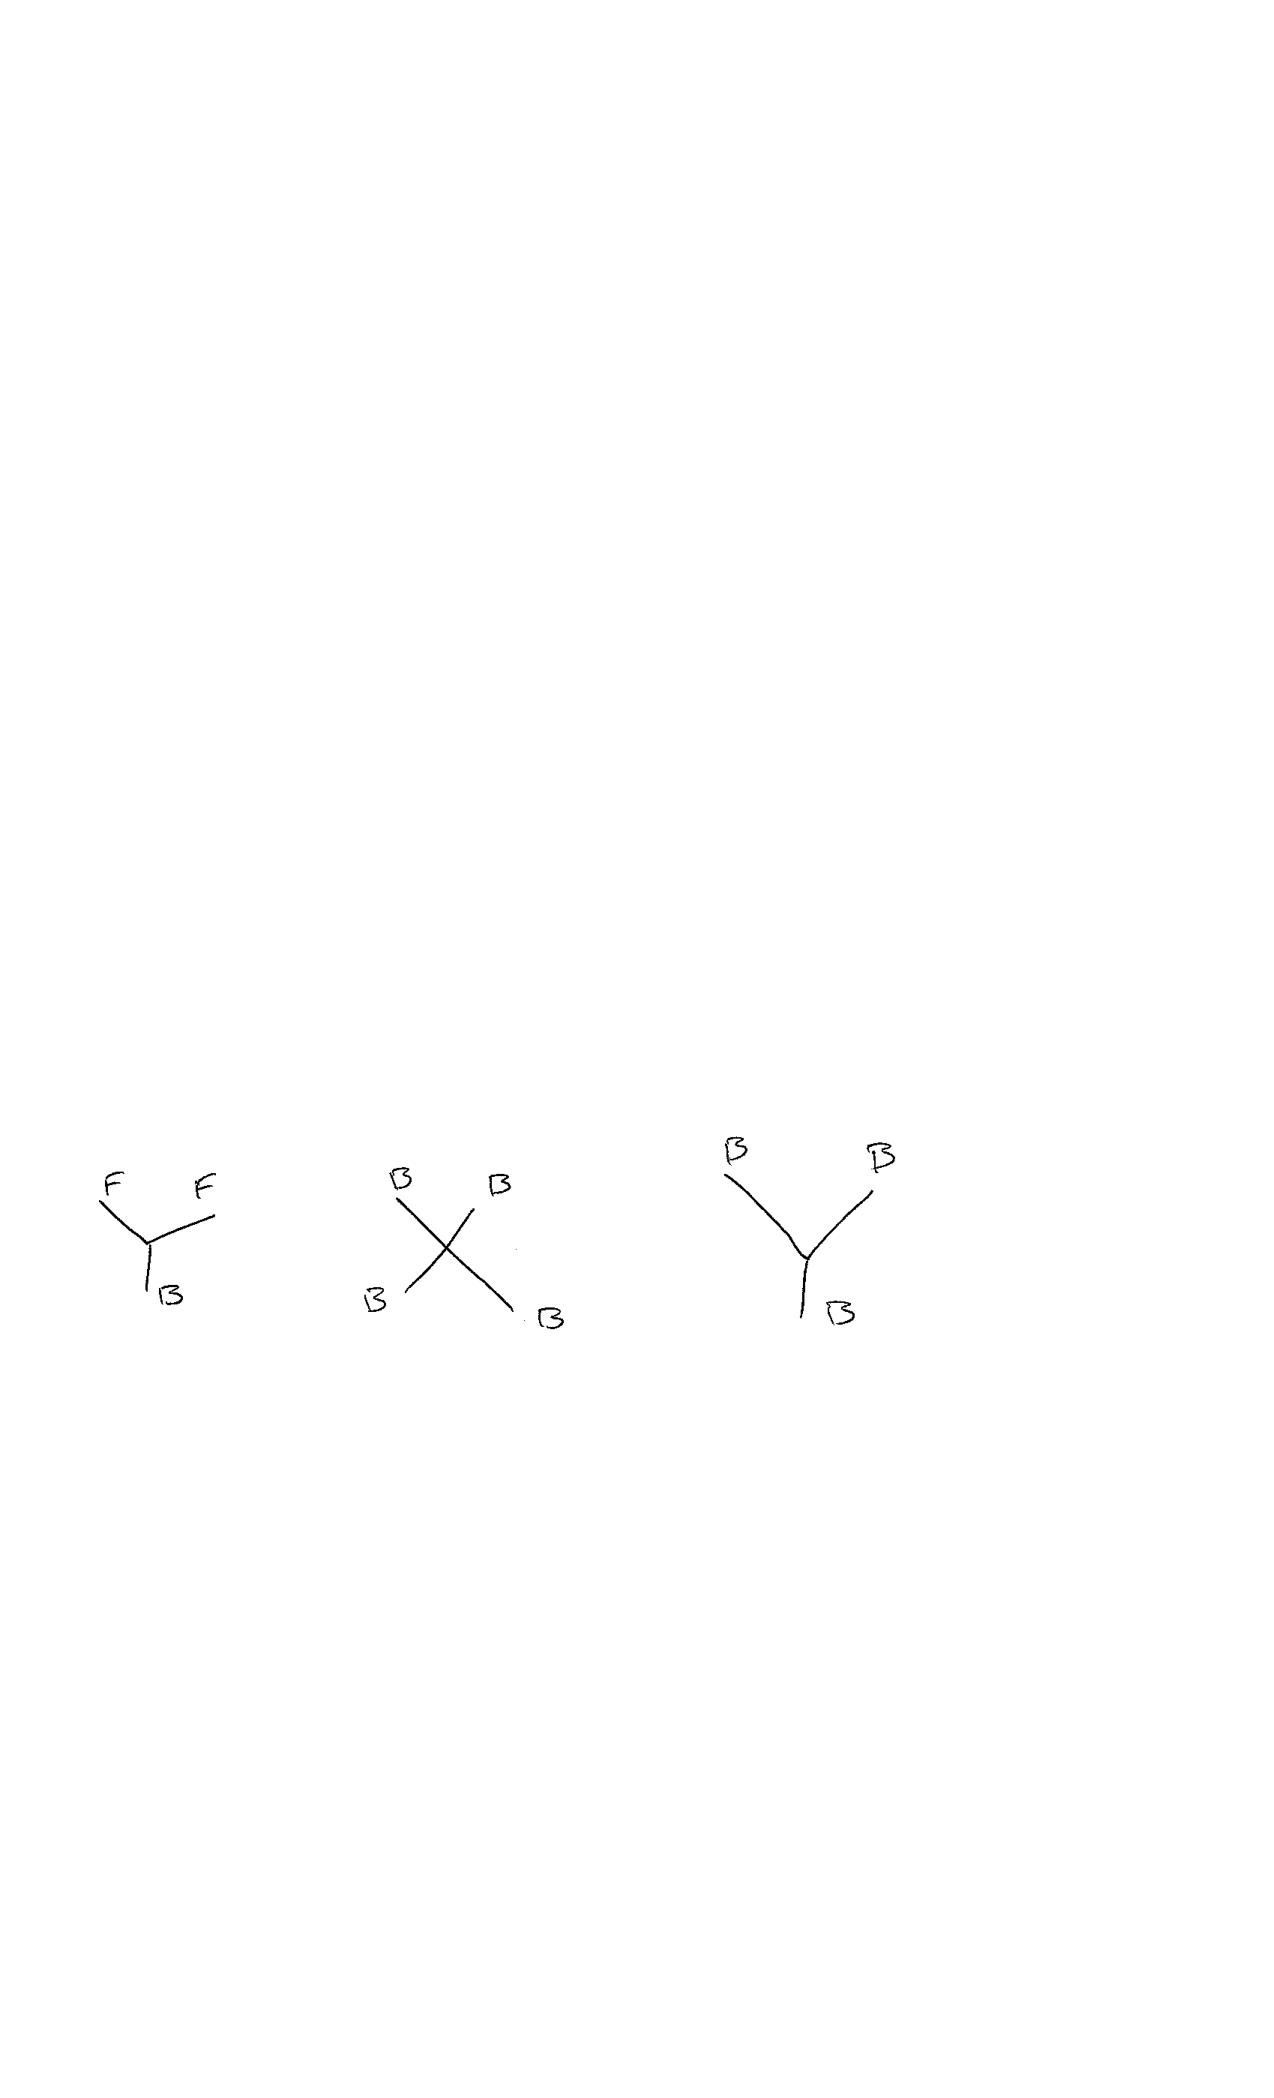
\includegraphics[width=0.9\textwidth]{../Week5_Lagrangians/Interactions.pdf}
\end{figure}

Spin-1 must be Yang-Mills (ect)

SM attempts to explain all phenomena of particle physics in terms of small number of particles. 

Actually 4 different types

\underline{Leptons} Spin-1/2 (Left and Right handend fields) Experience Weak and EM interactions
\be
\begin{pmatrix} \nu_e \\ e \end{pmatrix} \hspace*{0.1in} \begin{pmatrix} \nu_\mu \\ \mu \end{pmatrix} \hspace*{0.1in}  \begin{pmatrix} \nu_\tau \\ \tau \end{pmatrix}  
\ee

\underline{Quarks} Spin-1/2 Strong, Weak and EM interactions
\be
 \begin{pmatrix} u \\ d \end{pmatrix} \hspace*{0.1in}   \begin{pmatrix} c \\ s \end{pmatrix} \hspace*{0.1in}   \begin{pmatrix} t \\ b \end{pmatrix}
\ee

\underline{Gauge Bosons} Spin-1  Force Carriers
\be
 \gamma \hspace*{0.2in}   g (\times 8) \hspace*{0.2in} W^{\pm}  \hspace*{0.2in} Z
\ee

\underline{Higgs Boson} Spin-0  
\be
  H
\ee

All are assumed to be elementary.  No internal structure.

\underline{Leptons}

Quantum Number associated with each generation. 

eg: 

\be
L_e \equiv N(e^-) - N(e^+) + N(\nu_e) - N(\bar{\nu_e})
\ee

All other particles has $L_e = 0$.

Electron number is a conserved quantity.

$\Rightarrow$ electrons ($\nu_e$) must be created/destroyed in pairs.


Corrisponding conserved lepton numbers for $\mu$s and $\tau$s.

\be
L_\mu  \hspace*{1in} L_\tau
\ee


Leptons masses (GeV):
  
\be
\begin{pmatrix} m_\nu \\ 10^{-3} \end{pmatrix} \hspace*{0.1in} \begin{pmatrix} m_\nu \\ 10^{-1} \end{pmatrix} \hspace*{0.1in}  \begin{pmatrix} m_\nu \\ 1.7 \end{pmatrix}  
\ee

Note: $\sum m_\nu < 10^{-9} GeV$

Once thought to be 0.  Now known that at least 2 (maybe all) have $m_\nu > 0$.

\clearpage

\underline{W/Z Exchange}

EM mediated by the exchange of a photon.

\bc
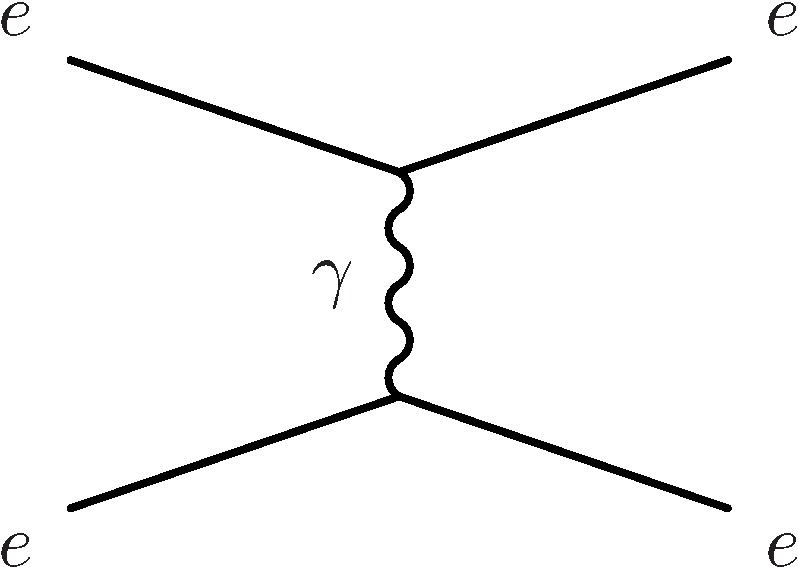
\includegraphics[width=0.4\textwidth]{./ElectronScattering.pdf}
\ec


Similarly for the weak interaction, force mediated by $W^{\pm}$ or Z.

When drawing diagrams, must remember to conserve Lepton numbers and EM charge.

eg: 

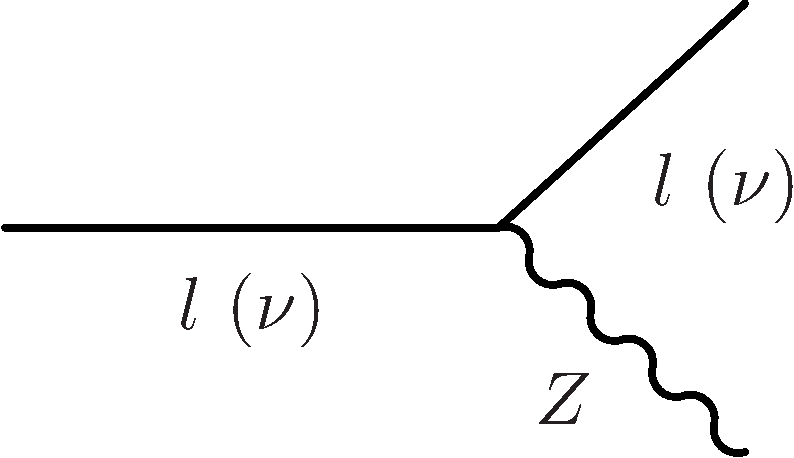
\includegraphics[width=0.25\textwidth]{./ZVertex.pdf}  \hfill 
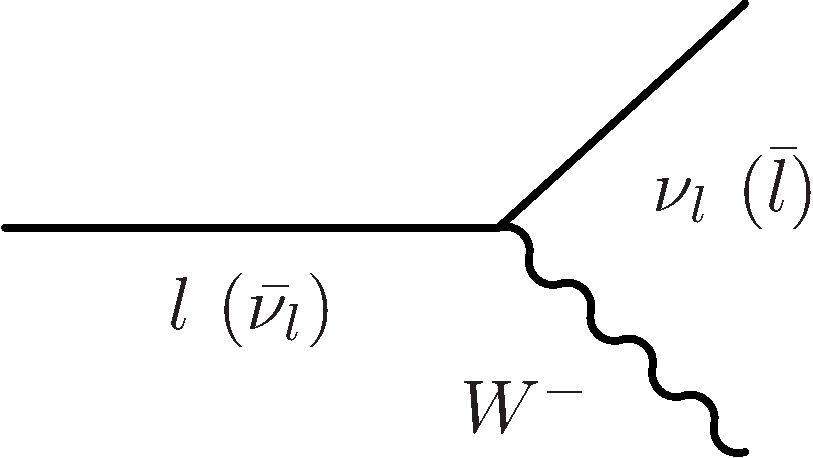
\includegraphics[width=0.25\textwidth]{./Wminus.pdf}   \hfill 
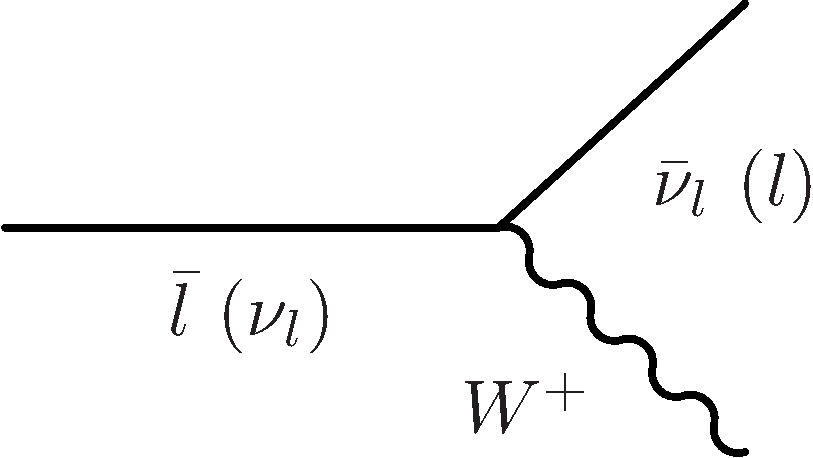
\includegraphics[width=0.25\textwidth]{./Wplus.pdf}   

eg:
\bc
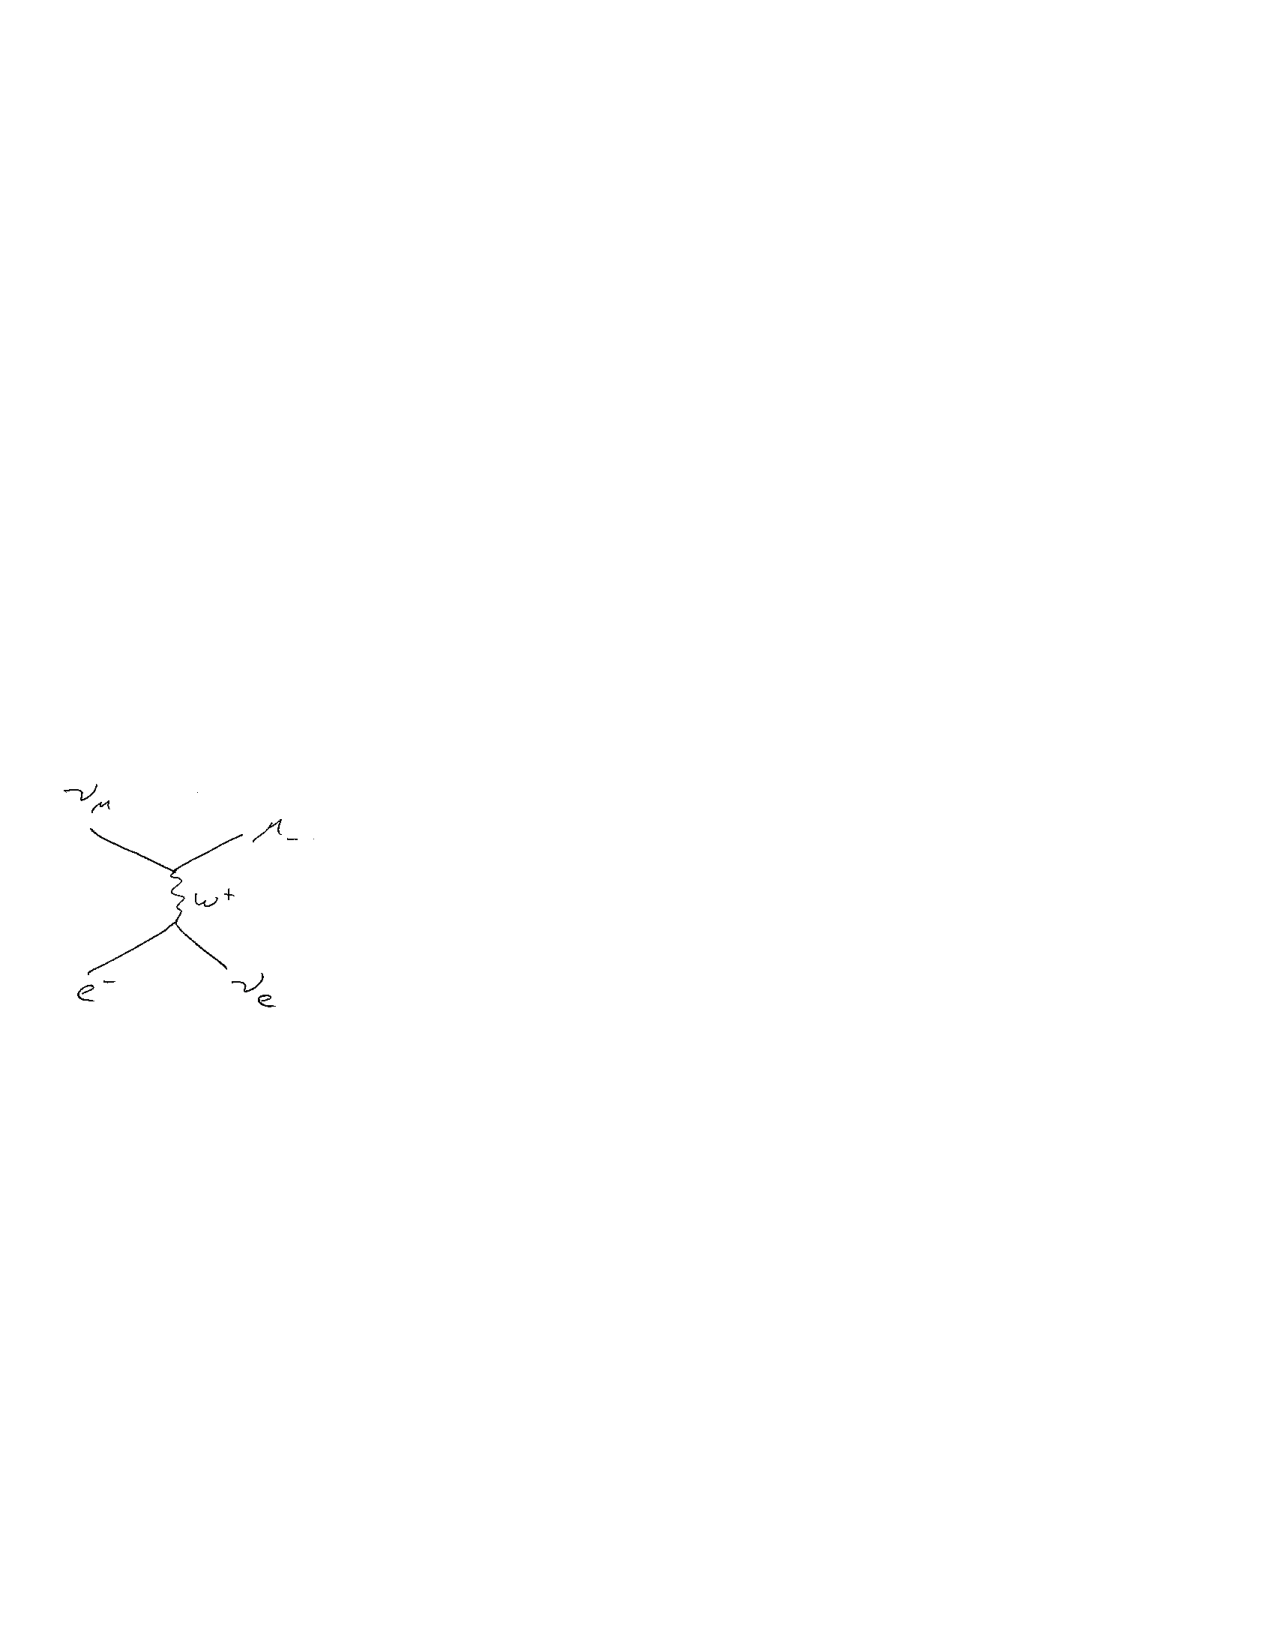
\includegraphics[width=0.3\textwidth]{./NuScattering.pdf}   
\ec

\underline{Lepton Universality}
All data consistent with hypothesis that interaction of all generations are the same.
(Modulo mass differences)

\clearpage


\bc
Now, $m_Z$ = 90 GeV and $m_W$ = 80 GeV  which $\ne$ 0 !
\ec

This has a major implication for the range, or effective strength of the interaction.


\begin{minipage}{0.4\textwidth}
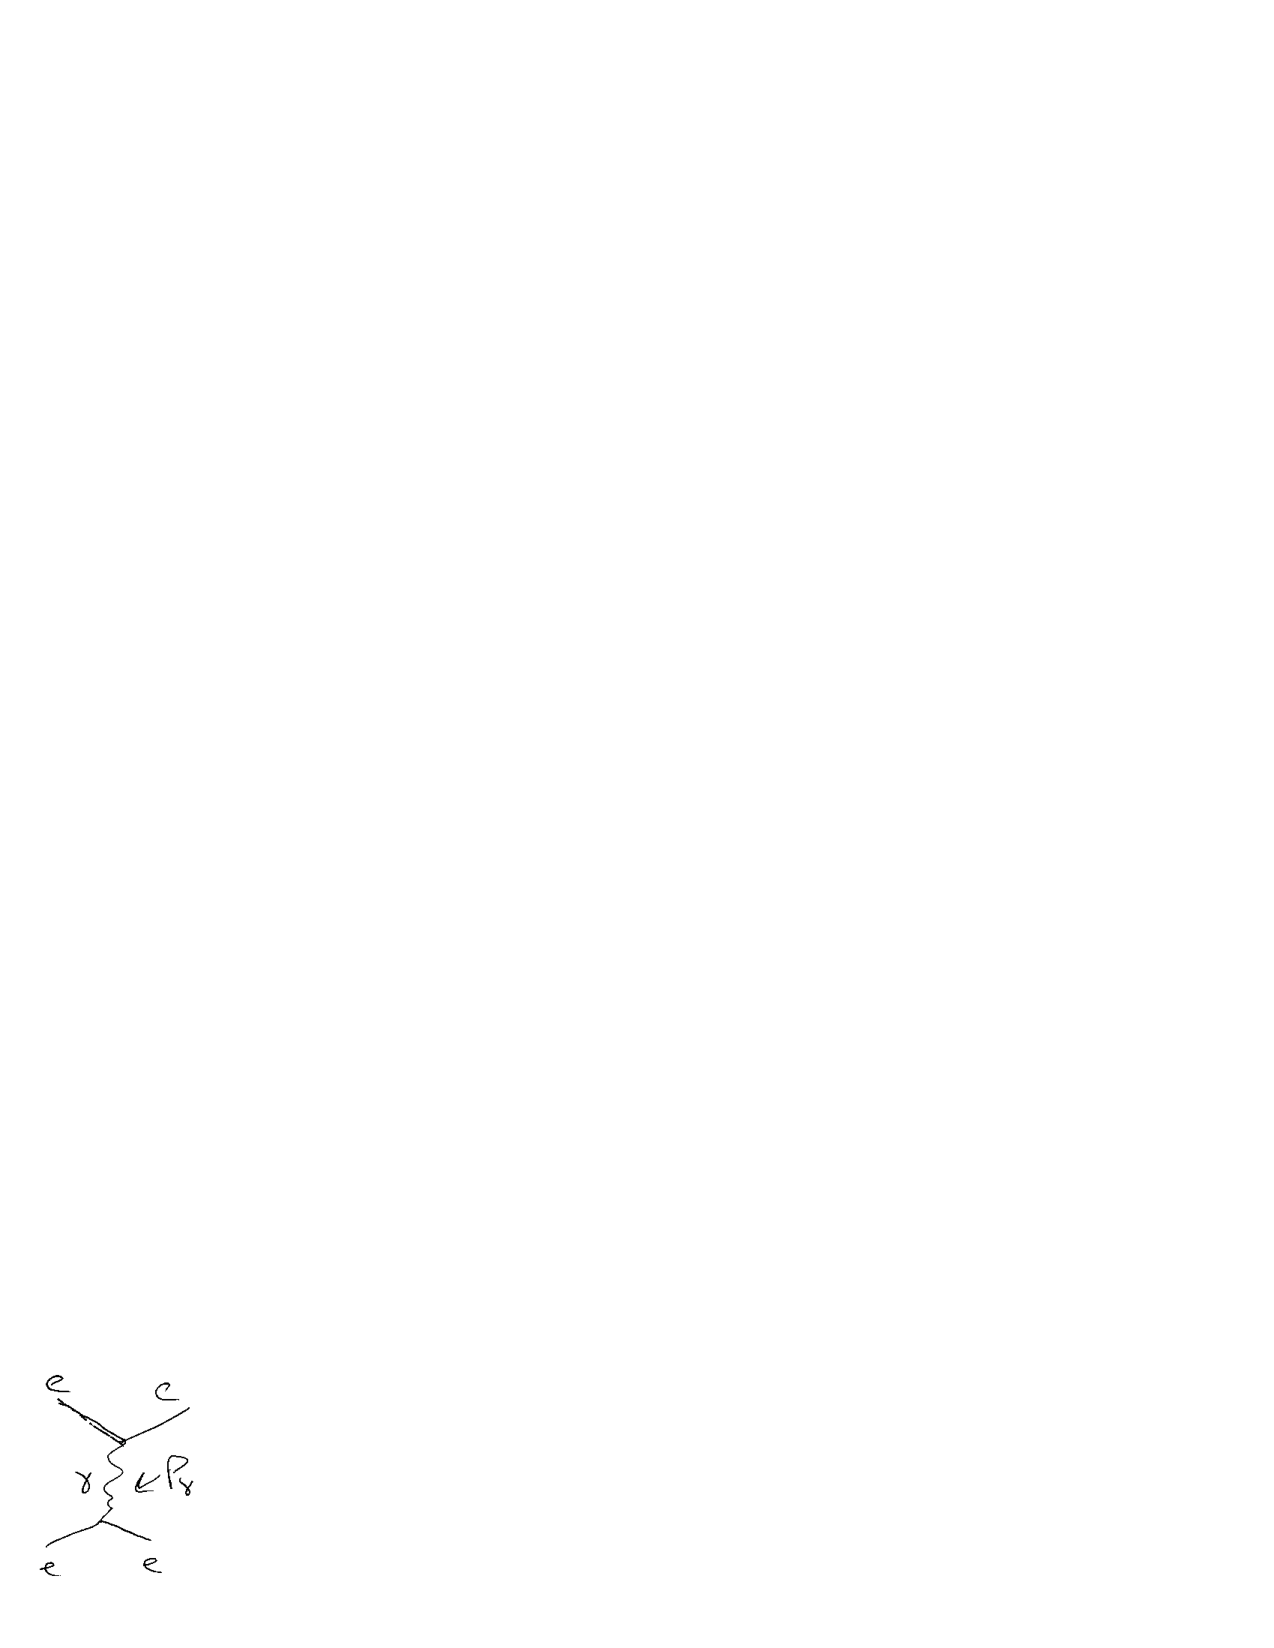
\includegraphics[width=0.8\textwidth]{./eeGamma.pdf}   
\end{minipage} %\hfill
\begin{minipage}{0.45\textwidth}
By uncertianty principle 
\bea
E \times t \sim 1 \\
E \times x \sim 1 \\
x \sim \frac{1}{E} \\ 
x \sim \frac{1}{p_\gamma}
\eea
$\frac{1}{p_\gamma}$ can be arbitrarily large for small $p_\gamma$.
\end{minipage} %\hfill



However, for the weak interaction. 

\begin{minipage}{0.4\textwidth}
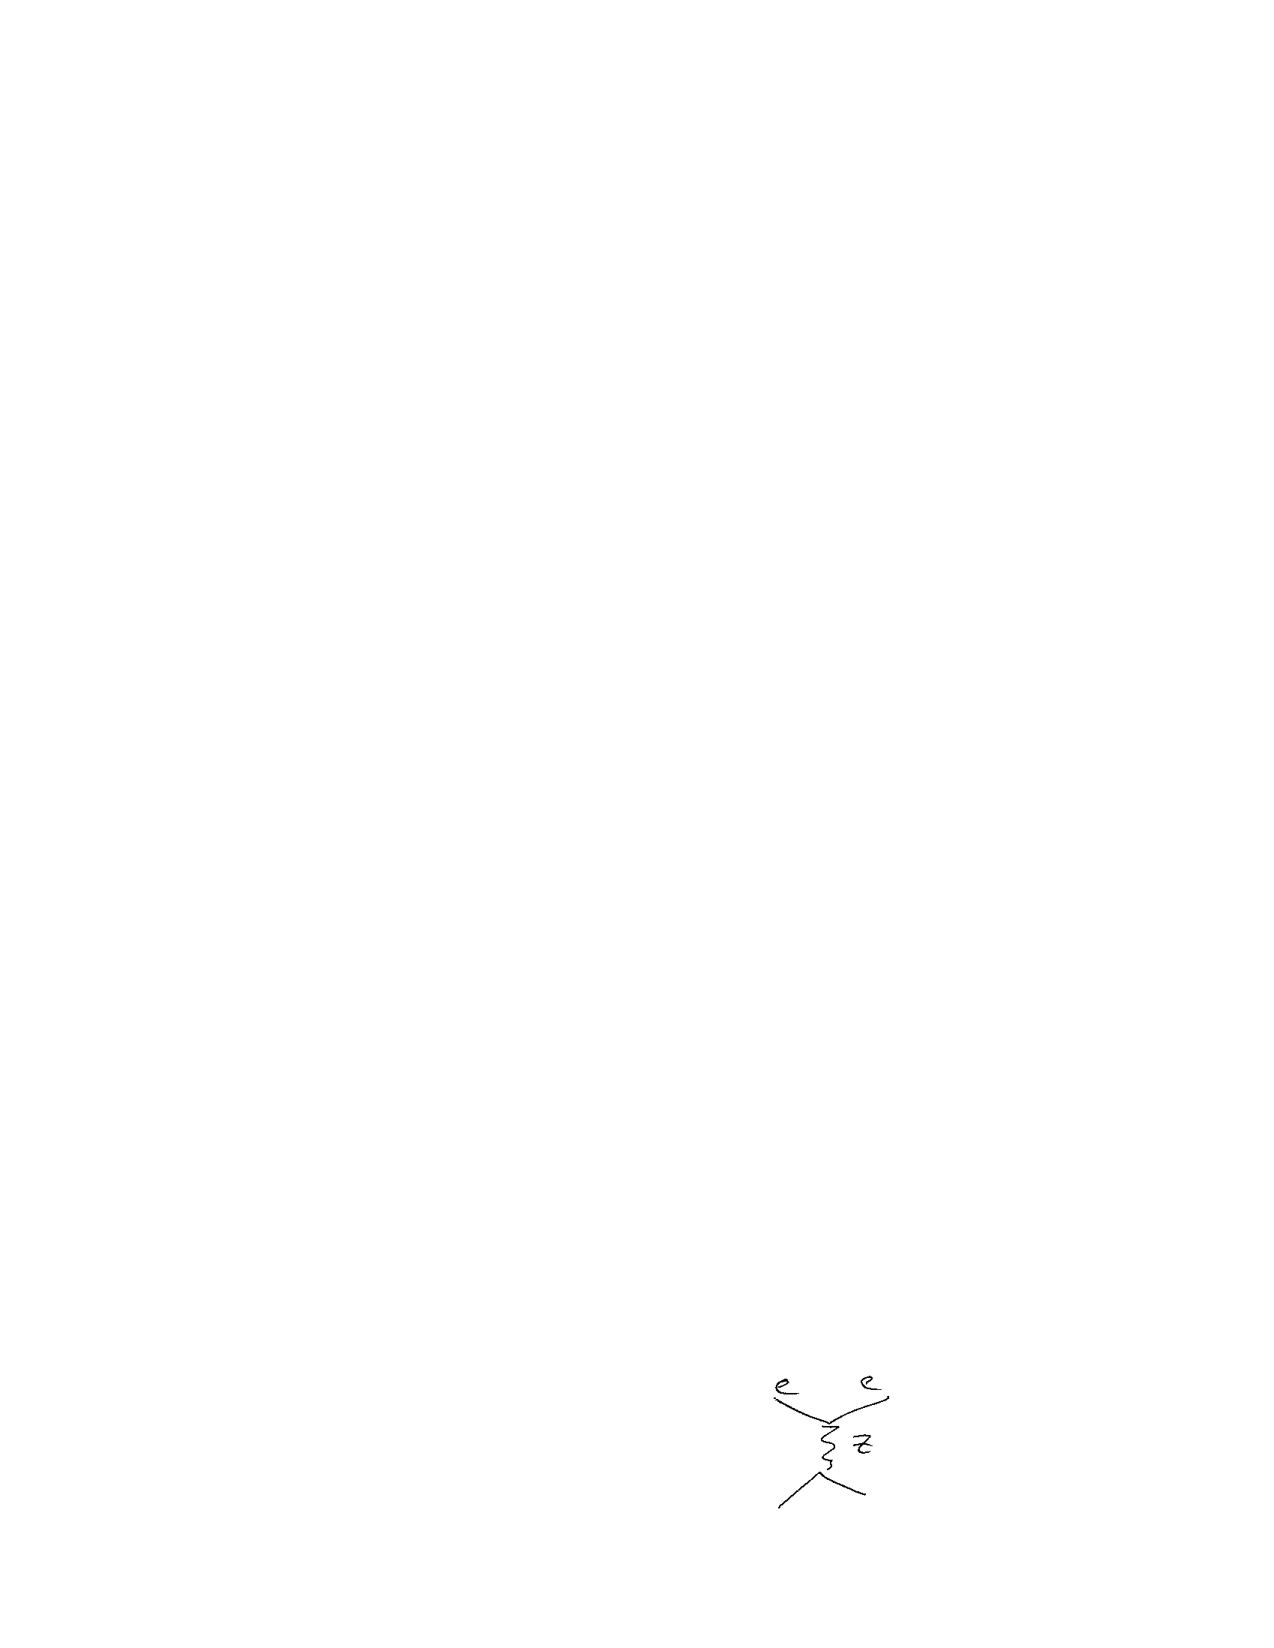
\includegraphics[width=0.8\textwidth]{./eeZScattering.pdf}   
\end{minipage} %\hfill
\begin{minipage}{0.45\textwidth}
\bea
x \sim \frac{1}{E_z} \sim \frac{1}{\sqrt{p_z^2 + m_z^2}} 
\eea
At max can be of range $\frac{1}{m_z}$
\end{minipage} %\hfill

At low energies the wavelengths of all particles are large compared  to the range of the wak force ($\frac{1}{m_Z}$)

\clearpage

Can be approximated by a \multiline{0-range \\ ``point''} interaction, whose strength is characterized by the ``Fermi constant'' 

\begin{center}
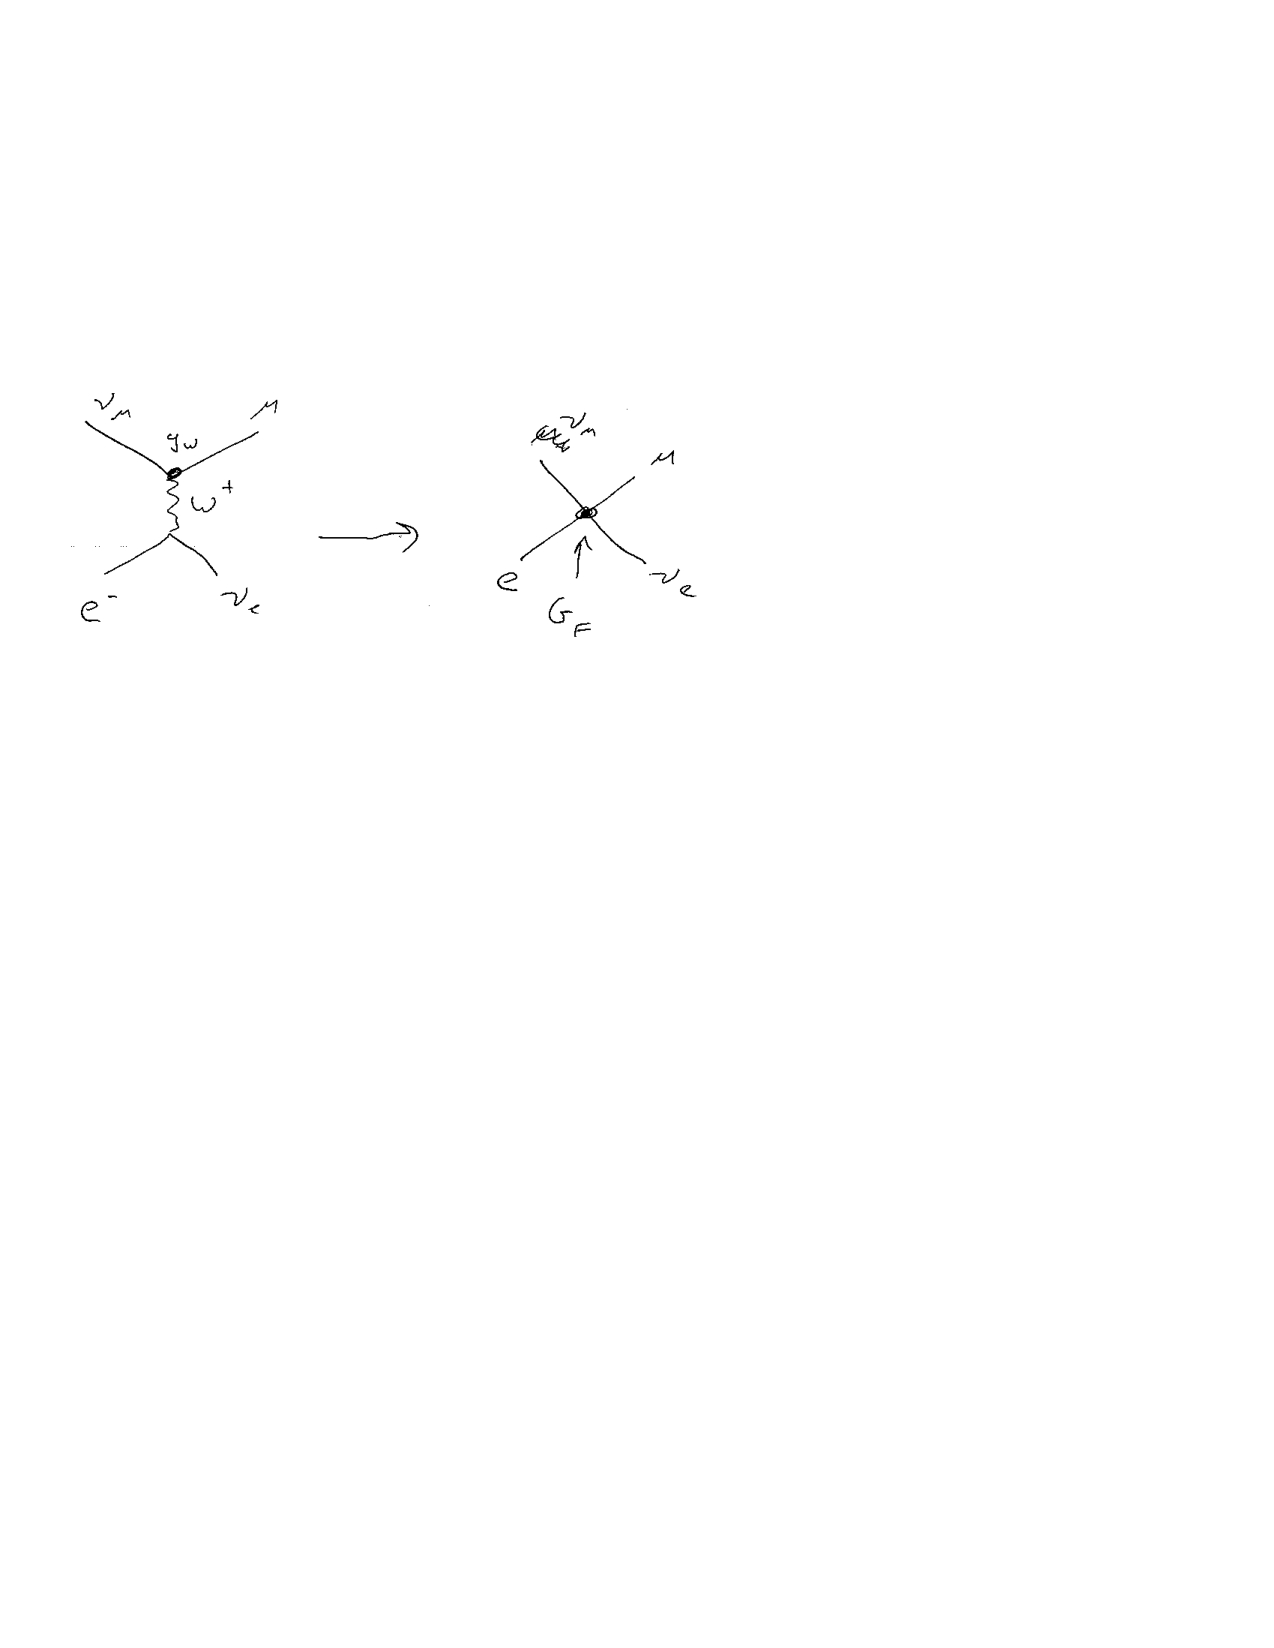
\includegraphics[width=0.6\textwidth]{./GFermi.pdf}   
\end{center}
\bea
G_F &\sim& 10^{-5}\ \GeV^{-2}\\
    &=& \frac{g_W^2}{m_W^2}\\
    &=& \frac{4\pi\alpha_W^2}{m_W^2}
\eea
where $\alpha_W = 4.26 \times 10^{-3} \sim 0.5 \alpha_{EM}$

Weak and EM interactions of similar strength. 

The apparent difference between Weak and EM interaction is a long distance \underline{illusion}.       

\underline{\underline{Branching Ratios}}

\be
\rmt{Br}(Z\rightarrow ll) = \frac{\Gamma(Z\rightarrow ll)}{\Gamma_{\rmt{total}}}
\ee

where $\Gamma(Z\rightarrow ll)$ is the decay rate $\Gamma = \frac{1}{2E}|M|^2d\Pi_{LIPS}$

and $\Gamma_{\rmt{total}} = \sum_i \Gamma(Z\rightarrow XX)$ 

\bea
\frac{\rmt{Br}(Z\rightarrow ee)}{\rmt{Br}(Z\rightarrow \mu\mu)} = \frac{\Gamma(Z\rightarrow ee)}{\Gamma(Z\rightarrow \mu\mu)} = \frac{\frac{1}{2E}|M(Z\rightarrow ee)|^2d\Pi_{LIPS}}{\frac{1}{2E}|M(Z\rightarrow \mu\mu)|^2d\Pi_{LIPS}} &=&  \frac{|M(Z\rightarrow ee)|^2}{|M(Z\rightarrow \mu\mu)|^2} \\
&=& \underbrace{1}_{\rmt{by lepton universality}}
\eea

}
\end{document}

